\chapter{提案手法}\label{proposed}
\ref{cnn-problem},\ref{gradcam-problem}で述べた問題点を解決するための手法を提案する.はじめに\ref{makedataset}節でGTZANデータセットを修正し,学習用データセットを作成する.次に\ref{classify-model}節で楽曲ジャンルを分類するモデルを構築し,\ref{generate-model}節で学習済みの分類モデルを用いて,スペクトログラムを生成するモデルを構築する.最後に\ref{visualize}節で,生成モデルを用いてジャンル境界を可視化する手法を述べる.

\section{データセットの作成}\label{makedataset}

\subsection{GTZANデータセットの修正}
本研究では,楽曲データセットとしてGTZANを使用する.GTZANデータセットは\figref{fig:gtzan}のようにBlues, Country, Classical, Disco, Hip-hop, Jazz, Metal, Pop, Reggae, Rockの10ジャンルの楽曲から構成される.各ジャンルを説明した表は\tabref{tab:genres}に示す\cite{genres}.
1データ当たりは30秒間の楽曲データであり,1ジャンルにつき100曲ずつ用意されている.GTZANデータセットには,ノイズデータや重複したデータが存在しているため,ノイズデータと重複した片方の楽曲データを除去する必要がある\cite{gtzanissue}.そのため最終的なデータセット数は\tabref{tab:gtzan}のようになった.
\begin{figure}[htbp]
	\begin{center}
		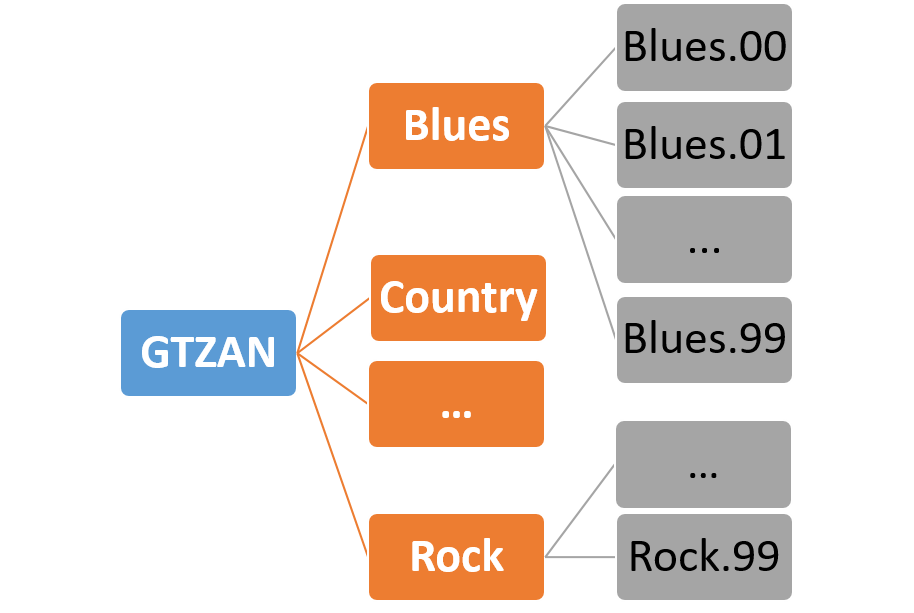
\includegraphics[scale=0.461]{./images/dataset/gtzan.png}
		\caption{GTZANデータセット}
		\label{fig:gtzan}
	\end{center}
\end{figure}

\begin{table}[htbp]
	\begin{center}
		\caption{各ジャンルの主な説明}
		\scalebox{0.91}{{}
			\begin{tabular}{|c||l|} \hline
				ジャンル & \hspace{190pt}説明  \\ \hline \hline
				Blues &  
				\begin{tabular}{l}
				米国深南部でアフリカ系アメリカ人の間から発生した音楽の一種およびその楽式.\\
				ギターを用いた歌が主役である.
				\end{tabular}\\ \hline
				Country & 
				\begin{tabular}{l}
				1920年代にアメリカ合衆国南部で発祥したとされる音楽.シンプルなハーモニーを\\
				形成し,バラードからダンス音楽まで幅広い音楽性を持つ. 
				\end{tabular}\\ \hline
				Classical &  
				\begin{tabular}{l}
				バロック音楽,古典派音楽,ロマン派音楽に当たる1550年頃から1900年頃の音楽.
				\end{tabular}\\ \hline
				Disco & 
				\begin{tabular}{l}
				一定のリズムを刻む4つ打ち,8分音符ないし16分音符刻みかつオフビートで\\
				オープンするハイハットパターンがある音楽.さらに突出したシンコペーション\\
				を持ったり,時にはオクターブでなるエレキベースのベースラインの上で演奏される.
				\end{tabular} \\ \hline
				Hip-hop & 
				\begin{tabular}{l}
				1970年代のアメリカ合衆国ニューヨークのブロンクス区で,アフロ・アメリカンや\\
				カリビアン・アメリカン,ヒスパニック系の住民のコミュニティで行われていた\\
				ブロックパーティから生まれた音楽.MCによるラップを乗せた音楽形態\\
				を指すことが一般化している.
				\end{tabular}\\ \hline
				Jazz & 
				\begin{tabular}{l}
				19世紀末から20世紀初頭にかけてアメリカ合衆国南部の都市を中心に派生した音楽.\\
				演奏の中にブルー・ノート,シンコペーション,スウィング,コールアンド\\
				レスポンス,即興演奏,ポリリズムなどの要素を組み込んでいることが\\
				大きな特徴とされている.
				\end{tabular}\\ \hline
				Metal &
				\begin{tabular}{l}
				ギター,ドラム,ボーカル,ベースを主軸とし,一般的には音の「ヘヴィさ」\\
				を重視した音楽.そのためにギターやベースのチューニングを下げ,\\
				通常より低い音が出せるようにしている場合もある. 
				\end{tabular}\\ \hline
				Pop & 
				\begin{tabular}{l}
				1950年代から1960年代にかけて西洋でロックンロールから派生して\\
				現代的形態で始まったポピュラー音楽.動きのあるメロディが重視され,\\
				基本的な楽式を楽曲中で繰り返すといった普遍的な特徴を持つ.
				\end{tabular}\\ \hline
				Reggae & 
				\begin{tabular}{l}
				ジャマイカで成立したポピュラー音楽全般.4分の4拍子の第2・第4拍目を\\
				カッティング奏法で刻むギター,	各小節の3拍目にアクセントが置かれるドラム,\\
				うねるようなベースラインを奏でるベースなどの音楽的特徴を持つ.
				\end{tabular}\\ \hline
				Rock & 
				\begin{tabular}{l}
				1950年代にアメリカ合衆国の黒人音楽であるRocknrollやBlues,Countryを起源\\
				とし,1960年代以降にイギリスやアメリカ合衆国で幅広く多様な様式へと展開した\\
				音楽.サウンドは伝統的にエレクトリックギターが中心となる.
				\end{tabular}\\ \hline
		\end{tabular}
		}
		\label{tab:genres}
	\end{center}
\end{table}

\begin{table}[htbp]
	\begin{center}
		\caption{ジャンル毎のデータセット数}
		\scalebox{0.91}{{}
			\begin{tabular}{|c|c|c|} \hline
				ジャンル & データセット数  \\ \hline
				Blues & 100 \\ \hline
				Country & 100 \\ \hline
				Classical & 100 \\ \hline
				Disco & \color{red}94 \\ \hline
				Hip-hop & \color{red}98 \\ \hline
				Jazz & \color{red}87 \\ \hline
				Metal & \color{red}91\\ \hline
				Pop & \color{red}91 \\ \hline
				Reggae & \color{red}89 \\ \hline
				Rock & 100  \\ \hline
		\end{tabular}
		}
		\label{tab:gtzan}
	\end{center}
\end{table}


\subsection{学習用データセット作成}
一般に音を分析するために使用されるデータとしては,音信号をSTFTした周波数情報が用いられる.そのため,楽曲ジャンルを分類においても,どの周波数がどの程度含まれるかということが重要であると考えられる.さらに楽曲という点でリズムとメロディーが存在するため,パーカッション成分とハーモニー成分に分けて分析することがより良い特徴が得られると考えられる.そこで楽曲をパーカッション成分とハーモニー成分に分けた周波数振幅スペクトログラムを生成する\cite{percuss_harmony}.\\
また,人間の聴覚に合わせた周波数がさらに効果的であると考えられるため,楽曲を周波数振幅スペクトログラムに変換した後,メルスケールに直したメル周波数スペクトログラムを学習データとする.学習させる楽曲データの時間的な長さに関しては,Weibinらの研究により3秒間が一番良い結果を得ているため.それに倣い3秒間のスペクトログラムを用いる\cite{weibin}.
以上の点を踏まえて\figref{fig:makedataset}のように,学習に用いるデータセットを作成する.

\begin{figure}[htbp]
	\begin{center}
		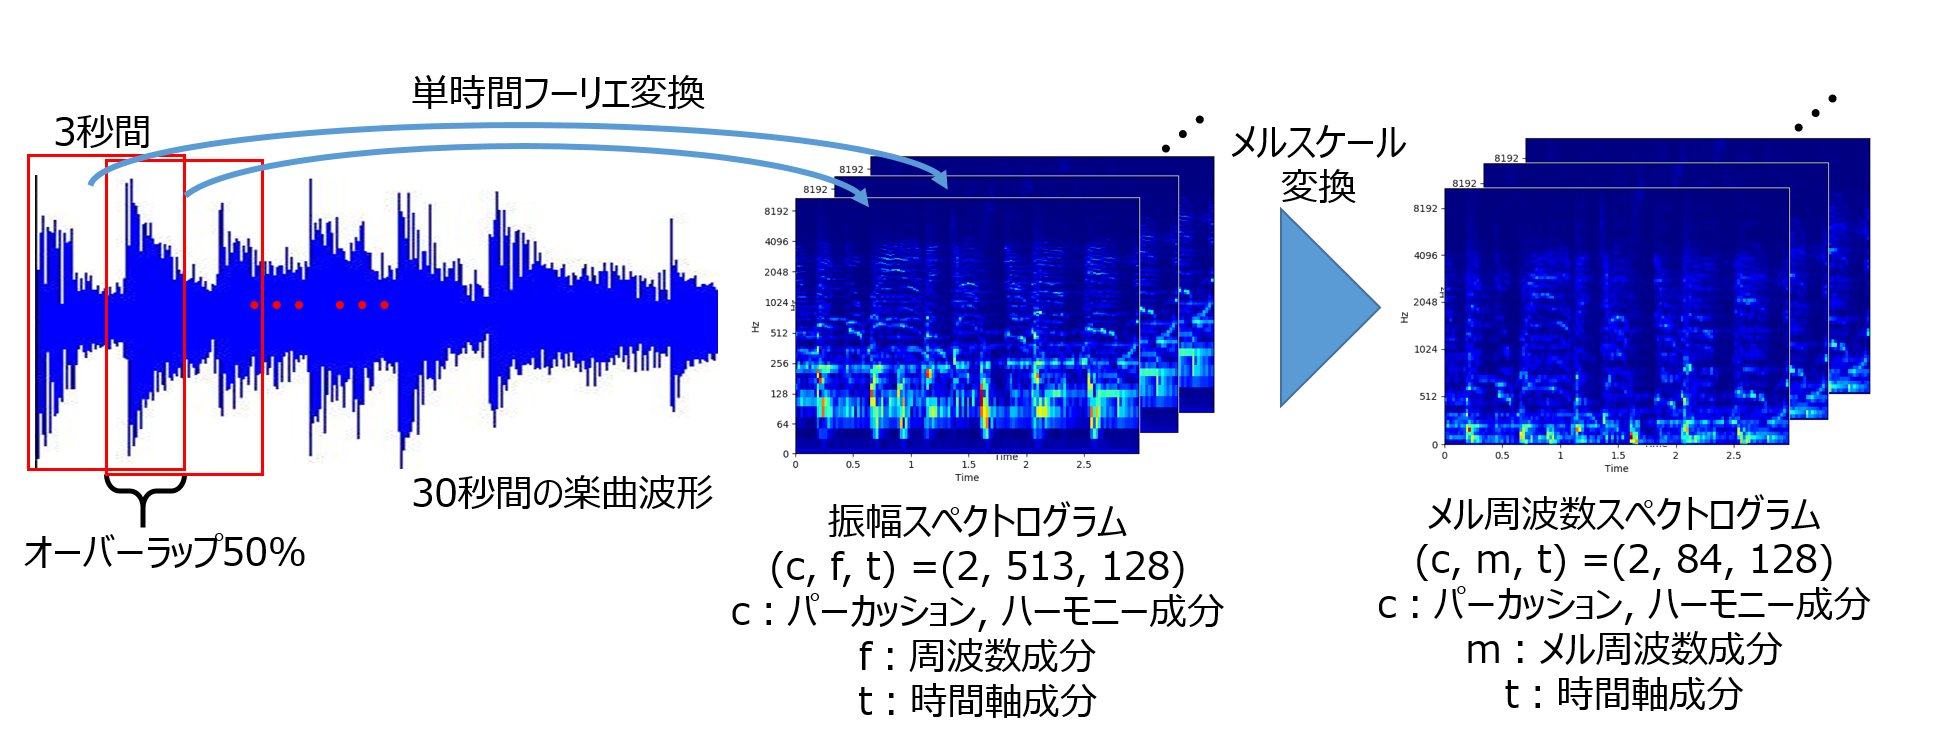
\includegraphics[scale=0.7]{./images/dataset/makedataset.png}
		\caption{学習データセット作成}
		\label{fig:makedataset}
	\end{center}
\end{figure}
ここで,データセットを増やすという目的で,STFTする際の窓のずらし方をオーバーラップを50\%として3秒間ごとに切り抜いていく.

また音量をバランスを統一するために3秒間の波形の振幅値を\eref{eq:normalize-sig}を用いて-1~1に正規化する.さらにモデルへの入力スケールを合わせるために,\eref{eq:normalize-mel}のように最大値で除算しメル周波数スペクトログラムの値を0~1の範囲で正規化する.
\begin{align}
	signal &= \frac{signal}{max(abs(signal))} \label{eq:normalize-sig}\\
	mel &= \frac{mel}{max(mel)} \label{eq:normalize-mel}
\end{align}


\clearpage
\section{ジャンル分類器の構築} \label{classify-model}
楽曲10ジャンルを分類する学習済みモデルを構築する.データセットは\ref{makedataset}節で述べたものを用いて,学習用データとテスト用データに分ける.

\subsection{ジャンル分類器}
\ref{makedataset}節で作成したスペクトログラムを用いて,\figref{fig:proposedCNN}のような入力をスペクトログラム,出力を楽曲10ジャンルに設定したCNNを分類器として構築する.CNNのネットワーク構成は\figref{fig:networkCNN}に示す.
なお学習時の損失関数は交差エントロピー誤差とする.
\begin{figure}[htbp]
	\begin{center}
		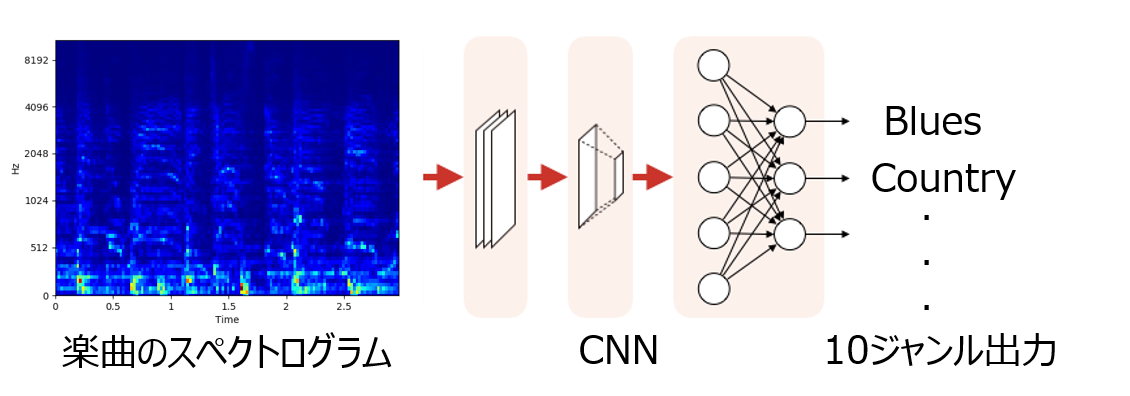
\includegraphics[scale=0.7]{./images/classify-model/proposedCNN.png}
		\caption{楽曲ジャンル分類モデル}
		\label{fig:proposedCNN}
	\end{center}
\end{figure}

\begin{figure}[htbp]
	\begin{center}
		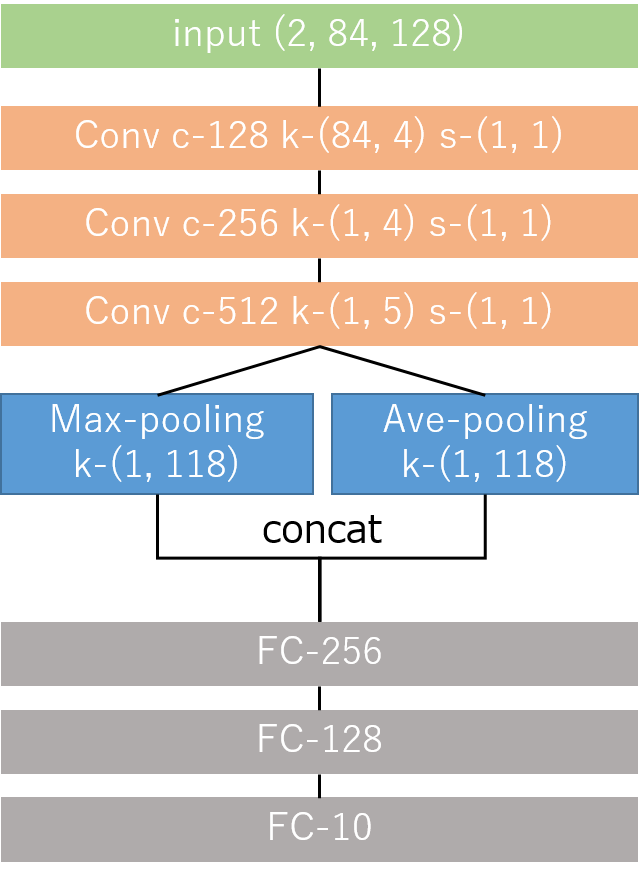
\includegraphics[scale=0.425]{./images/classify-model/network.png}
		\caption{CNNのネットワーク構成}
		\label{fig:networkCNN}
	\end{center}
\end{figure}



\newpage
\section{データ生成器の構築}\label{generate-model}
\ref{classify-model}節で構築した学習済みCNNを用いて,ジャンル毎で異なるデータを生成するようなモデルを構築する.本稿で構築した生成器は$-$1~1の一様分布に従うランダムノイズを入力とし,メル周波数スペクトログラムを出力する.さらに生成されたスペクトログラムを学習済CNNによって分類する.このときノイズベクトルの値を連続的に変化させることで,生成データの連続変化とジャンル出力の連続変化が同時に確認できる.
\figref{fig:proposed-abst}はデータ生成器を学習する際の全体像を示しており,\figref{fig:proposed-abst2}は学習後に使用するモデルの全体像を示した図である.

\vspace{30pt}
\begin{figure}[htbp]
	\begin{center}
		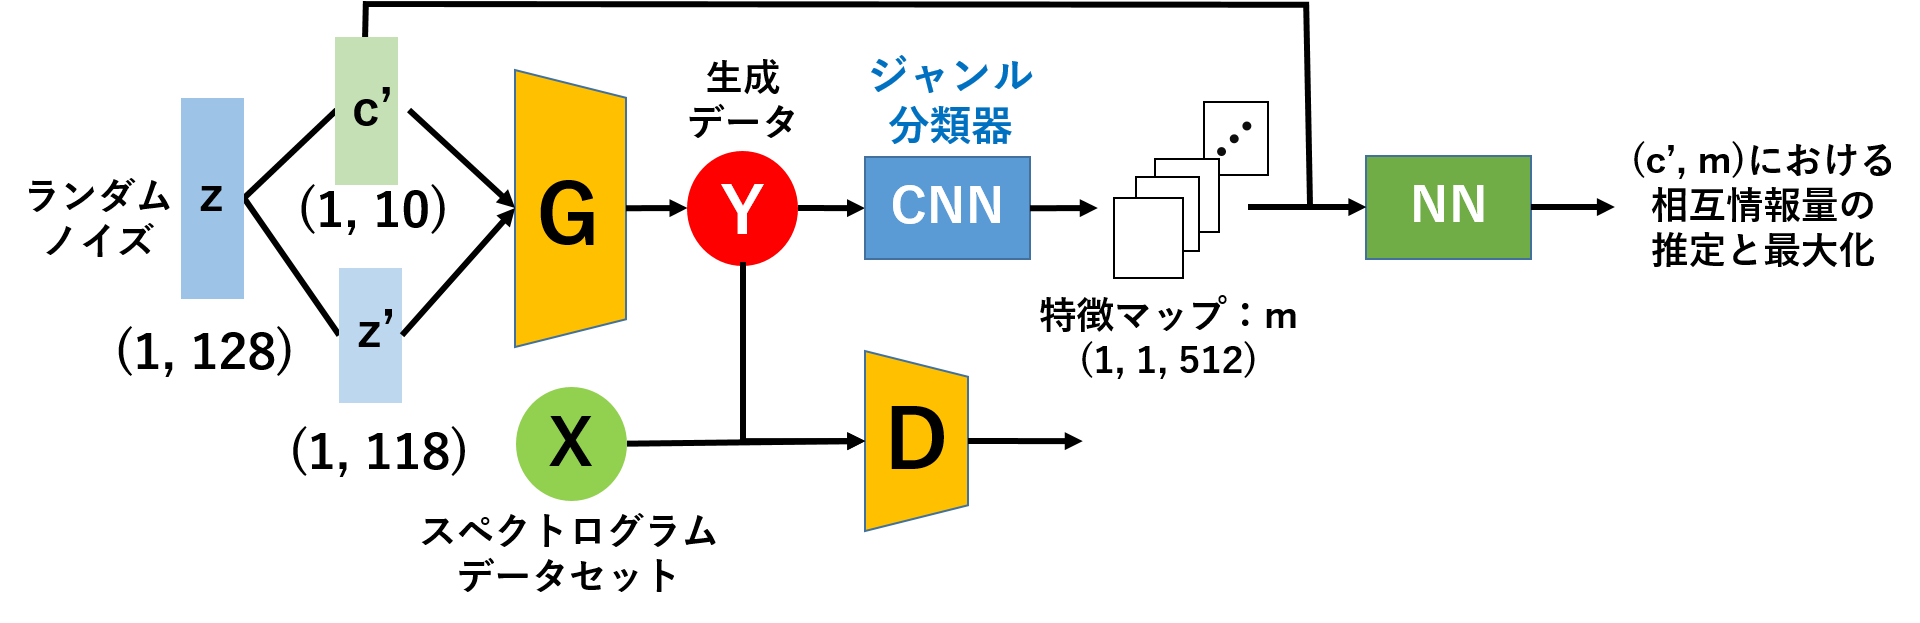
\includegraphics[scale=0.5]{./images/generate-model/abst.png}
		\caption{データ生成器の学習}
		\label{fig:proposed-abst}
	\end{center}
\end{figure}
\begin{figure}[htbp]
	\begin{center}
		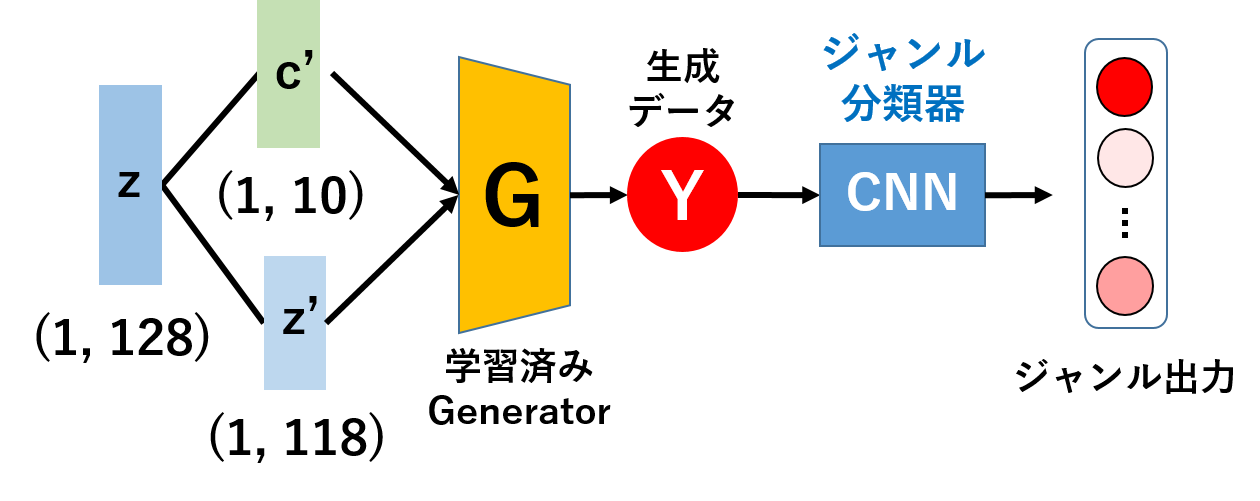
\includegraphics[scale=0.5]{./images/generate-model/abst2.png}
		\caption{生成データの分類}
		\label{fig:proposed-abst2}
	\end{center}
\end{figure}


\clearpage
\subsection{生成器モデル}
\figref{fig:proposedgan}のようなGANモデルを構築する.$-$1~1の一様分布に従うランダムノイズをGeneratorに入力し,Generatorが出力したデータとGTZANデータセットのスペクトログラムをDiscriminatorによって判定する.これにより生成するデータをスペクトログラムに近づけていく.使用するGeneratorとDiscriminatorのネットワーク構成を\figref{fig:network-gan-gen}と\figref{fig:network-gan-dis}に示す.


Generatorの入力されるノイズベクトルの次元は128次元であり,全結合層で次元を増加させ,逆畳み込みによって最終的にデータセットのメル周波数スペクトログラムと同じ次元の(2, 84, 128)の配列を出力する.一方Discriminatorの入力はデータセット配列またはGeneratorによって生成された配列を入力とし,畳み込み層で特徴マップを得たのち全結合層によって1次元の値まで次元が縮小されていく.この1次元の出力値がWasserstein距離となる.

\begin{figure}[htbp]
	\begin{center}
		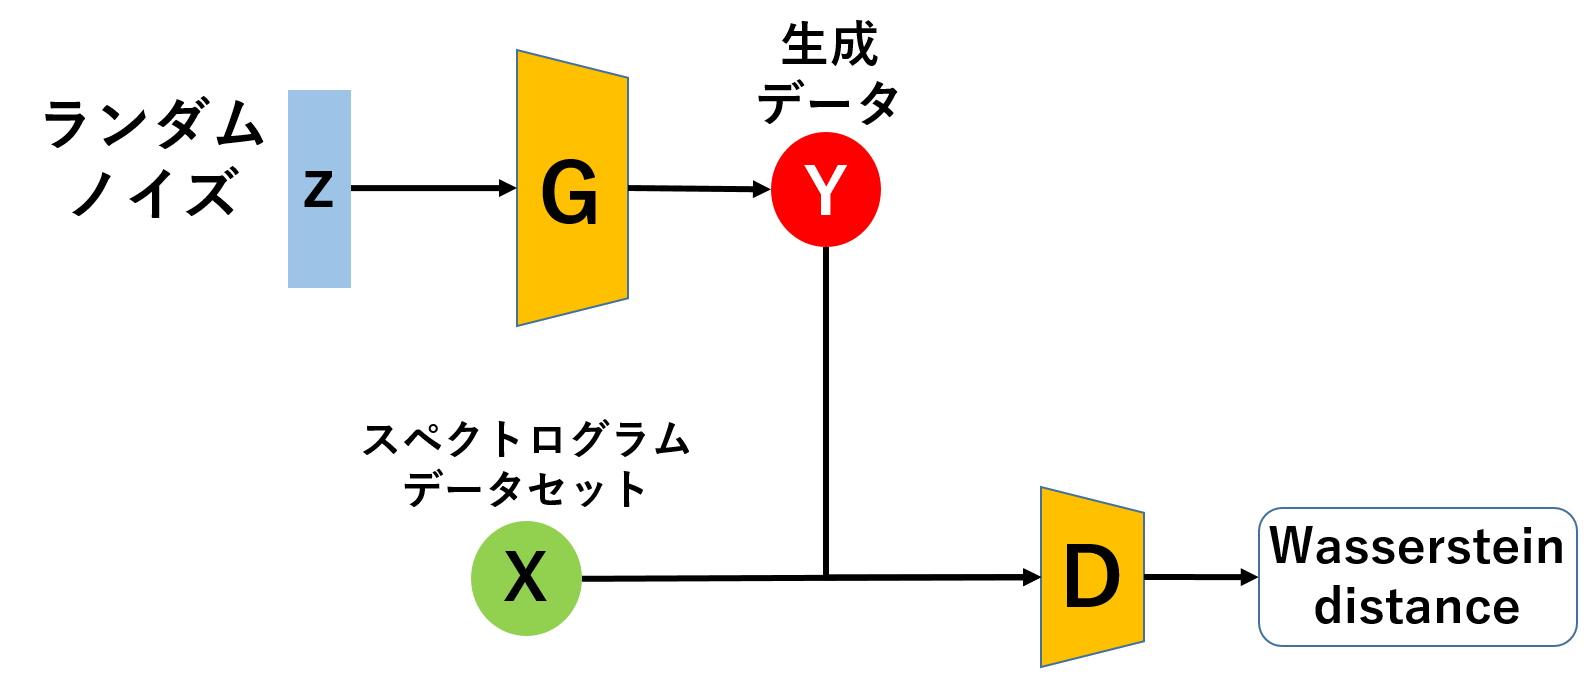
\includegraphics[scale=0.58]{./images/generate-model/proposed_gan.png}
		\caption{生成器モデル}
		\label{fig:proposedgan}
	\end{center}
\end{figure}

\begin{figure}[htbp]
	\begin{center}
		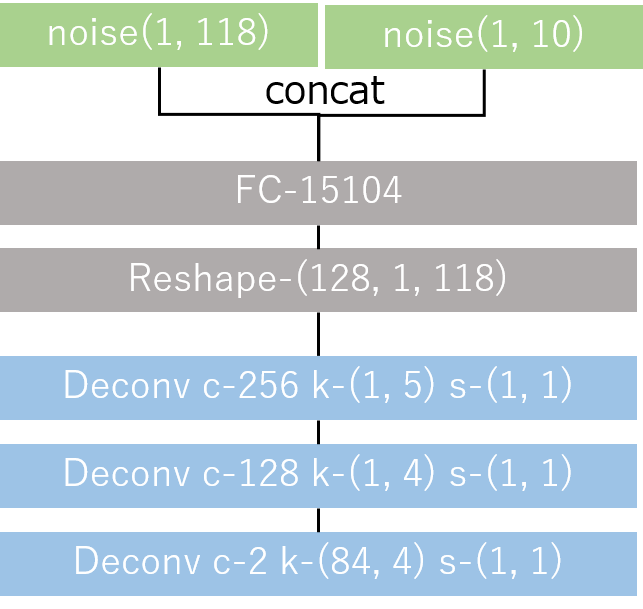
\includegraphics[scale=0.7]{./images/generate-model/generator.png}
		\caption{Generatorのネットワーク構成}
		\label{fig:network-gan-gen}
	\end{center}
\end{figure}

\begin{figure}[htbp]
	\begin{center}
		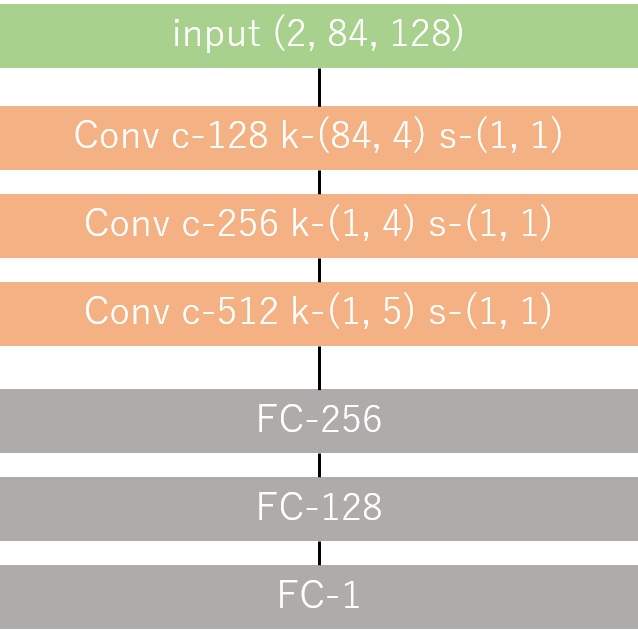
\includegraphics[scale=0.7]{./images/generate-model/discriminator.png}
		\caption{Discriminatorのネットワーク構成}
		\label{fig:network-gan-dis}
	\end{center}
\end{figure}

\clearpage
\subsection{ランダムノイズと分類結果の従属性}
生成データの分類結果と,Generatorの入力ランダムノイズに従属関係を持たせたい.そこで,NNを用いた相互情報量を推定し最大化する手法を用いる.\figref{fig:continuous}のようにGeneratorの入力ランダムノイズの128次元ベクトルを118次元と10次元のベクトルに分け,10次元のベクトル$c$とCNNのプーリング後の特徴マップ$m$との間に,相互情報量を推定し最大化するようなNNの学習を行う.これにより10次元の入力ベクトルと出力される特徴マップとの間に従属関係ができるため,特徴マップ後の全結合層の推論にも影響を与える.よってGeneratorの入力変数値とジャンル出力値が互いに影響しあうようなモデルが構築できる.また,\figref{fig:continuous}におけるNNのネットワーク構成を\figref{fig:network-continuous}に示す.
\begin{figure}[htbp]
	\begin{center}
		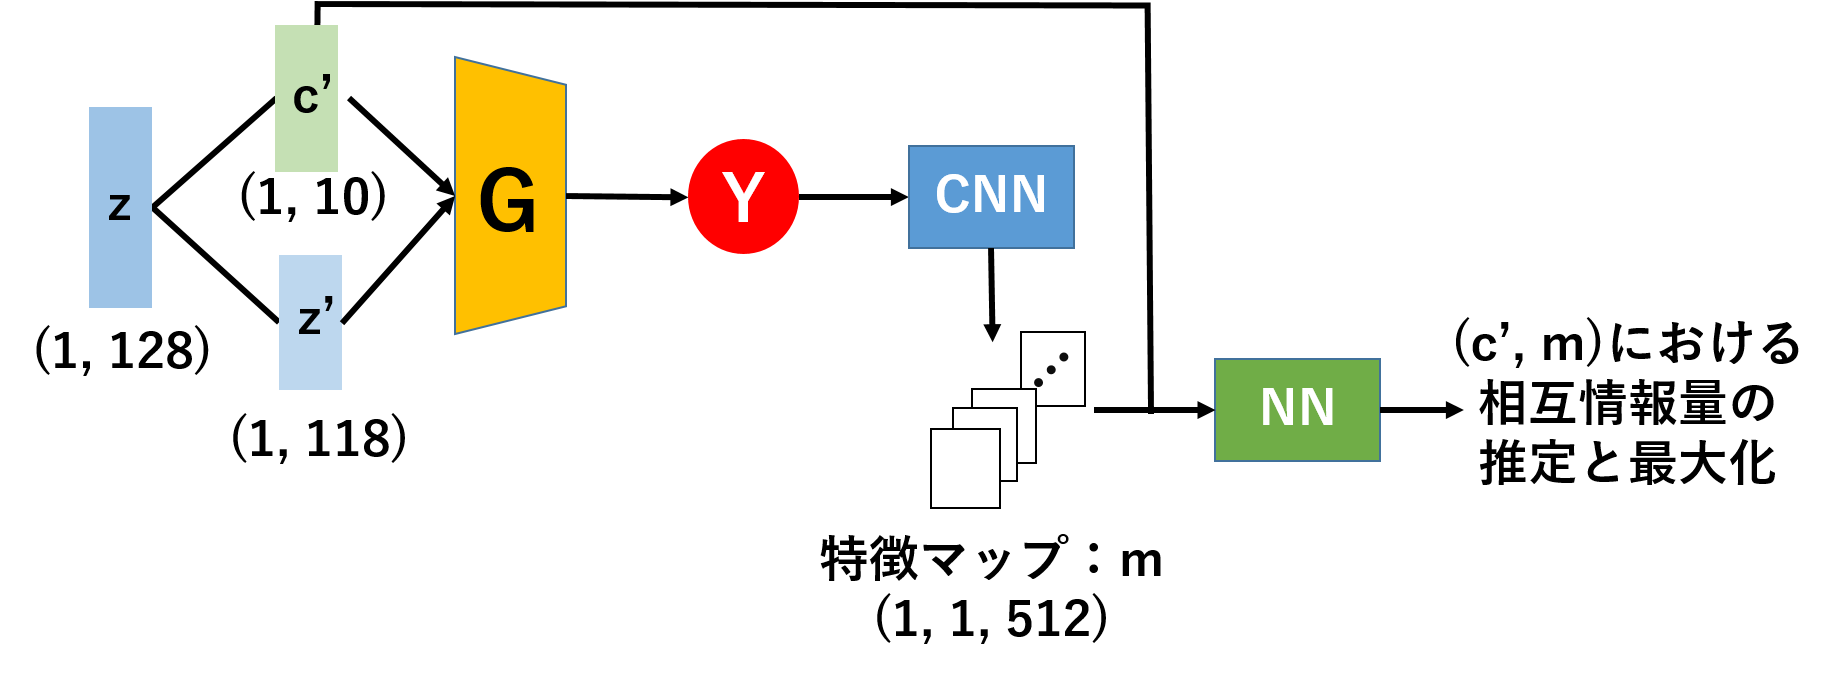
\includegraphics[scale=0.68]{./images/generate-model/continuous_gan.png}
		\caption{相互情報量の推定と最大化}
		\label{fig:continuous}
	\end{center}
\end{figure}
\begin{figure}[htbp]
	\begin{center}
		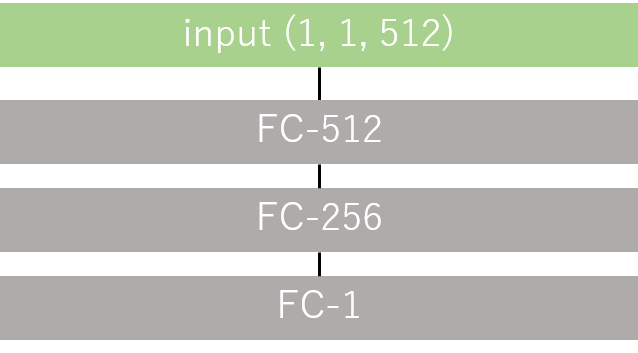
\includegraphics[scale=0.48]{./images/generate-model/continuous.png}
		\caption{NNのネットワーク構成}
		\label{fig:network-continuous}
	\end{center}
\end{figure}


\clearpage
\section{ジャンル境界の可視化}\label{visualize}
\ref{generate-model}節で構築した学習済みGeneratorを用いて,入力ノイズベクトルとジャンル出力の関係を二次元ジャンルマップ空間として可視化する.これにより,ジャンル間の境界を可視化することに加えスペクトログラムも生成することができるため,ジャンルにまたがったスペクトログラムの変化の過程を追うことができ,分類器がどのようにジャンルを分けているかという点において人間が意味解釈をする際の手助けとなる.


\figref{fig:randomnoise}のように初めに初期値として$-$1~1の一様分布に従うランダムノイズを128次元生成する.次に\figref{fig:variablenoise}のように従属関係にある10次元のベクトル$c$から2次元だけを取り出しその値を変化させいく.このとき,値の変換に応じて生成するスペクトログラムとジャンル分類結果が変化するため,その時の2次元ベクトルの値とジャンル分類結果を\figref{fig:featmap}のようにジャンルマップにプロットしていく.これにより,ジャンル境界となる座標が明らかとなる.

\begin{figure}[htbp]
	\begin{center}
		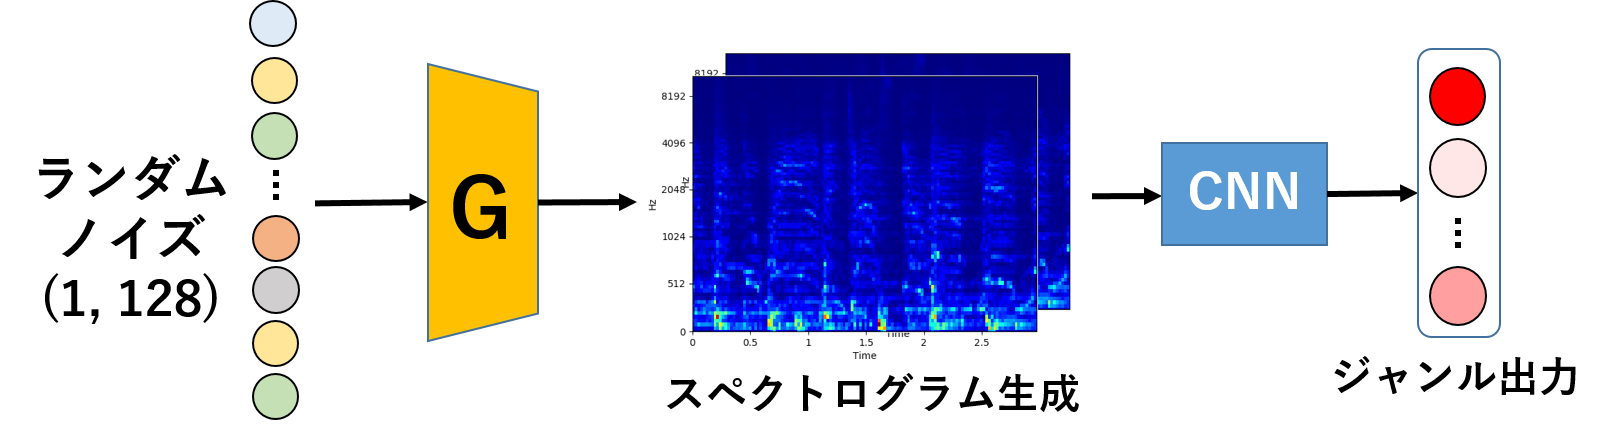
\includegraphics[scale=0.5]{./images/visualize/randomnoise.png}
		\caption{初期値ランダムノイズ生成}
		\label{fig:randomnoise}
	\end{center}
\end{figure}
\begin{figure}[htbp]
	\begin{center}
		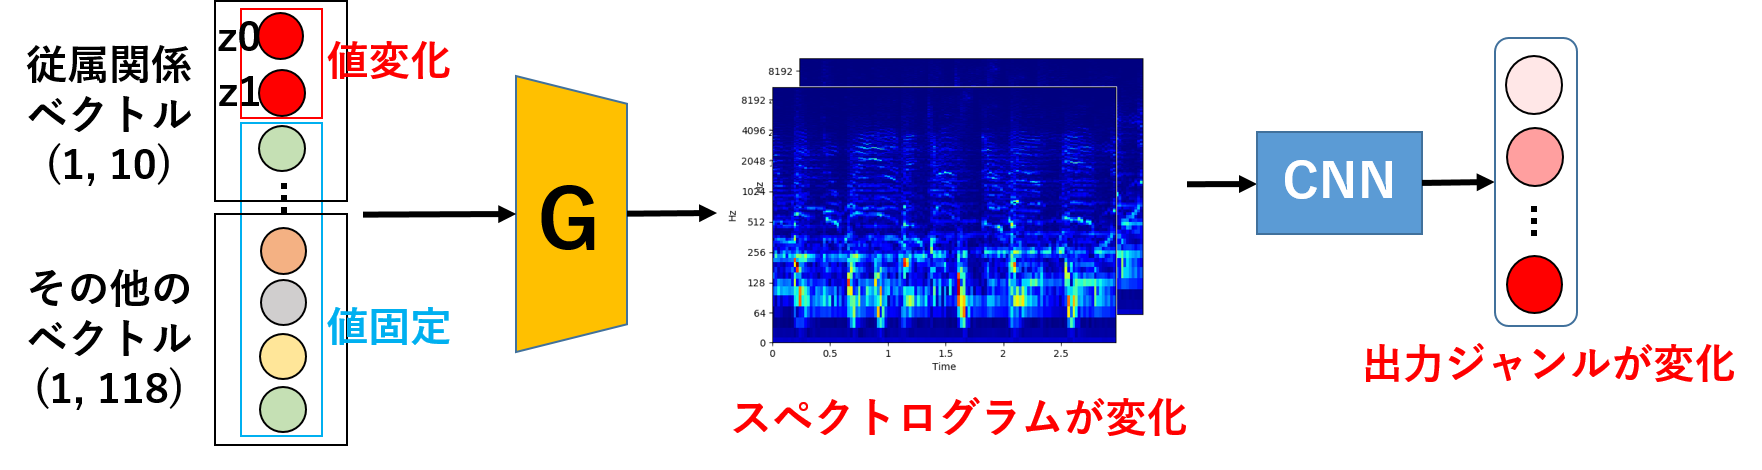
\includegraphics[scale=0.5]{./images/visualize/variablenoise.png}
		\caption{従属関係のベクトル値を変化}
		\label{fig:variablenoise}
	\end{center}
\end{figure}

\begin{figure}
	\begin{center}
		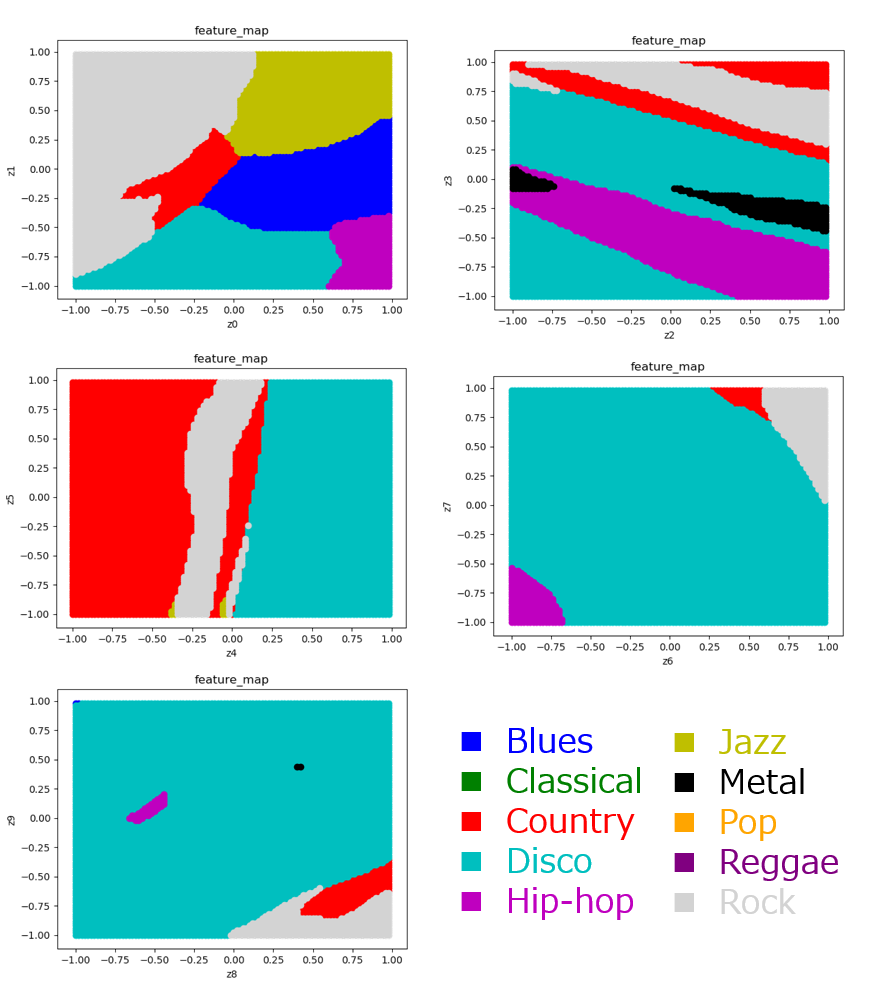
\includegraphics[scale=1]{./images/visualize/map0.png}
		\caption{軸ごとにおける2次元ジャンルマップの例}
		\label{fig:featmap}
	\end{center}
\end{figure}